\section{Multidimensional scaling}
\frame{\sectionpage}


\begin{frame}[fragile]{Multidimensional Scaling}

  \begin{itemize}
  \item Have distances between individuals.
  \item Want to draw a picture (map) in 2 dimensions showing
    individuals so that distances (or order of distances) as close
    together as possible. (Or maybe 3 with \texttt{rgl}.)
  \item If want to preserve actual distances, called {\em metric
      multidimensional scaling} (in R, \texttt{cmdscale}).
  \item If only want to preserve order of distances, called {\em
      non-metric multidimensional scaling} (in R, \texttt{isoMDS} in
    package \texttt{MASS}).
  \item Metric scaling has solution that can be worked out exactly.
  \item Non-metric only has iterative solution.
  \item Assess quality of fit, see whether use of resulting map is
    reasonable. (Try something obviously 3-dimensional and assess its
    failure.)
  \end{itemize}

\end{frame}

\begin{frame}[fragile]{Packages}
  
  The usual, plus a new one:
  
\begin{knitrout}
\definecolor{shadecolor}{rgb}{0.969, 0.969, 0.969}\color{fgcolor}\begin{kframe}
\begin{alltt}
\hlkwd{library}\hlstd{(MASS)}
\hlkwd{library}\hlstd{(tidyverse)}
\end{alltt}


{\ttfamily\noindent\itshape\color{messagecolor}{\#\# Loading tidyverse: ggplot2\\\#\# Loading tidyverse: tibble\\\#\# Loading tidyverse: tidyr\\\#\# Loading tidyverse: readr\\\#\# Loading tidyverse: purrr\\\#\# Loading tidyverse: dplyr}}

{\ttfamily\noindent\itshape\color{messagecolor}{\#\# Conflicts with tidy packages ----------------------------------------------}}

{\ttfamily\noindent\itshape\color{messagecolor}{\#\# filter(): dplyr, stats\\\#\# lag():\ \ \ \ dplyr, stats\\\#\# select(): dplyr, MASS}}\begin{alltt}
\hlkwd{library}\hlstd{(ggrepel)}
\hlkwd{library}\hlstd{(ggmap)}
\end{alltt}


{\ttfamily\noindent\itshape\color{messagecolor}{\#\# Google Maps API Terms of Service: http://developers.google.com/maps/terms.}}

{\ttfamily\noindent\itshape\color{messagecolor}{\#\# Please cite ggmap if you use it: see citation("{}ggmap"{}) for details.}}\end{kframe}
\end{knitrout}
  
\end{frame}


\begin{frame}[fragile]{Metric scaling: European cities}

CSV file \verb-europe.csv- contains road distances (in km) between 16 European cities. Can we reproduce a map of Europe from these distances?

Read in data and examine:

\begin{knitrout}\scriptsize
\definecolor{shadecolor}{rgb}{0.969, 0.969, 0.969}\color{fgcolor}\begin{kframe}
\begin{alltt}
\hlstd{europe}\hlkwb{=}\hlkwd{read.csv}\hlstd{(}\hlstr{"europe.csv"}\hlstd{,}\hlkwc{header}\hlstd{=T,}\hlkwc{stringsAsFactors}\hlstd{=F)}
\hlkwd{head}\hlstd{(europe)}
\end{alltt}
\begin{verbatim}
##            X Amsterdam Athens Barcelona Berlin Cologne Copenhagen
## 1  Amsterdam         0   3082      1639    649     280        904
## 2     Athens      3082      0      3312   2552    2562       3414
## 3  Barcelona      1639   3312         0   1899    1539       2230
## 4     Berlin       649   2552      1899      0     575        743
## 5    Cologne       280   2562      1539    575       0        730
## 6 Copenhagen       904   3414      2230    743     730          0
##   Edinburgh Geneva London Madrid Marseille Munich Paris Prague Rome Vienna
## 1      1180   1014    494   1782      1323    875   515    973 1835   1196
## 2      3768   2692   3099   3940      2997   2210  3140   2198 2551   1886
## 3      2181    758   1512    628       515   1349  1125   1679 1471   1989
## 4      1727   1141   1059   2527      1584    604  1094    354 1573    666
## 5      1206    765    538   1776      1208    592   508    659 1586    915
## 6      1864   1531   1196   2597      1914   1204  1329   1033 2352   1345
\end{verbatim}
\end{kframe}
\end{knitrout}


\end{frame}


\begin{frame}[fragile]{Multidimensional scaling}

  \begin{itemize}
  \item Create distance object first using all but first column of
\texttt{europe}. \texttt{europe} has distances in it already, so make
into \texttt{dist} with \texttt{as.dist}.
\item Then run multidimensional scaling and look at result:
  
\begin{knitrout}
\definecolor{shadecolor}{rgb}{0.969, 0.969, 0.969}\color{fgcolor}\begin{kframe}
\begin{alltt}
\hlstd{europe.d}\hlkwb{=}\hlkwd{as.dist}\hlstd{(europe[,}\hlopt{-}\hlnum{1}\hlstd{])}
\hlstd{europe.scale}\hlkwb{=}\hlkwd{cmdscale}\hlstd{(europe.d)}
\hlkwd{head}\hlstd{(europe.scale)}
\end{alltt}
\begin{verbatim}
##                   [,1]      [,2]
## Amsterdam  -348.162277  528.2657
## Athens     2528.610410 -509.5208
## Barcelona  -695.970779 -984.6093
## Berlin      384.178025  634.5239
## Cologne       5.153446  356.7230
## Copenhagen -187.104072 1142.5926
\end{verbatim}
\end{kframe}
\end{knitrout}

\item This is a matrix of $x$ and $y$ coordinates for plotting.

  \end{itemize}
\end{frame}

\begin{frame}[fragile]{Make data frame and plot points labelled by city}
  
\begin{knitrout}\small
\definecolor{shadecolor}{rgb}{0.969, 0.969, 0.969}\color{fgcolor}\begin{kframe}
\begin{alltt}
\hlstd{d}\hlkwb{=}\hlkwd{data.frame}\hlstd{(europe.scale,}\hlkwc{city}\hlstd{=europe[,}\hlnum{1}\hlstd{],}
  \hlkwc{stringsAsFactors}\hlstd{=F)}
\hlkwd{head}\hlstd{(d)}
\end{alltt}
\begin{verbatim}
##                     X1        X2       city
## Amsterdam  -348.162277  528.2657  Amsterdam
## Athens     2528.610410 -509.5208     Athens
## Barcelona  -695.970779 -984.6093  Barcelona
## Berlin      384.178025  634.5239     Berlin
## Cologne       5.153446  356.7230    Cologne
## Copenhagen -187.104072 1142.5926 Copenhagen
\end{verbatim}
\end{kframe}
\end{knitrout}

\begin{itemize}
\item City names appear as row names, but we need actual named column.
  
\item Points to plot have gained names \texttt{X1}, \texttt{X2}.
  
\begin{knitrout}
\definecolor{shadecolor}{rgb}{0.969, 0.969, 0.969}\color{fgcolor}\begin{kframe}
\begin{alltt}
\hlstd{g}\hlkwb{=}\hlkwd{ggplot}\hlstd{(d,}\hlkwd{aes}\hlstd{(}\hlkwc{x}\hlstd{=X1,}\hlkwc{y}\hlstd{=X2,}\hlkwc{label}\hlstd{=city))}\hlopt{+}\hlkwd{geom_point}\hlstd{()}\hlopt{+}
  \hlkwd{coord_fixed}\hlstd{()}\hlopt{+}\hlkwd{geom_text_repel}\hlstd{()}
\end{alltt}
\end{kframe}
\end{knitrout}
\end{itemize}
  
\end{frame}

\begin{frame}[fragile]{The picture}
  
\begin{knitrout}
\definecolor{shadecolor}{rgb}{0.969, 0.969, 0.969}\color{fgcolor}\begin{kframe}
\begin{alltt}
\hlstd{g}
\end{alltt}
\end{kframe}
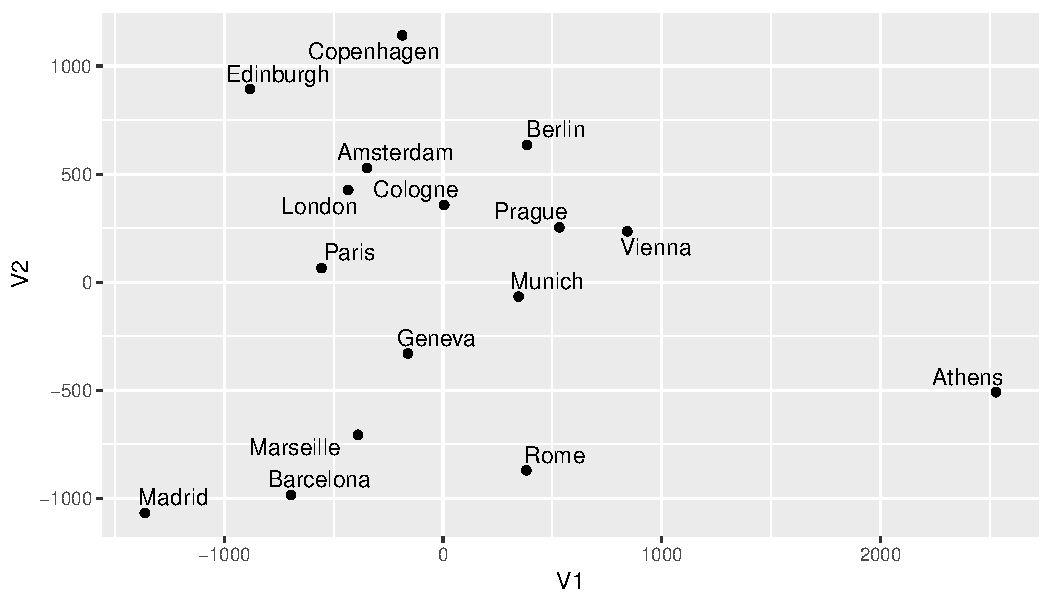
\includegraphics[width=\maxwidth]{figure/piaacenza-1} 

\end{knitrout}

  
\end{frame}

\begin{frame}[fragile]{Drawing a map of the real Europe}
  
  \begin{itemize}
  \item Works with package \texttt{ggmap}.
    
  \item First find latitudes and longitudes of our cities, called \emph{geocoding}:
    
\begin{knitrout}
\definecolor{shadecolor}{rgb}{0.969, 0.969, 0.969}\color{fgcolor}\begin{kframe}
\begin{alltt}
\hlstd{latlong}\hlkwb{=}\hlkwd{geocode}\hlstd{(d}\hlopt{$}\hlstd{city)}
\end{alltt}


{\ttfamily\noindent\color{warningcolor}{\#\# Warning in readLines(connect, warn = FALSE): URL 'https://maps.googleapis.com/maps/api/geocode/json?address=Amsterdam': status was 'Couldn't resolve host name'}}

{\ttfamily\noindent\color{warningcolor}{\#\# Warning in FUN(X[[i]], ...):\ \  geocoding failed for "{}Amsterdam"{}.\\\#\#\ \  if accompanied by 500 Internal Server Error with using dsk, try google.}}

{\ttfamily\noindent\color{warningcolor}{\#\# Warning in readLines(connect, warn = FALSE): URL 'https://maps.googleapis.com/maps/api/geocode/json?address=Athens': status was 'Couldn't resolve host name'}}

{\ttfamily\noindent\color{warningcolor}{\#\# Warning in FUN(X[[i]], ...):\ \  geocoding failed for "{}Athens"{}.\\\#\#\ \  if accompanied by 500 Internal Server Error with using dsk, try google.}}

{\ttfamily\noindent\color{warningcolor}{\#\# Warning in readLines(connect, warn = FALSE): URL 'https://maps.googleapis.com/maps/api/geocode/json?address=Barcelona': status was 'Couldn't resolve host name'}}

{\ttfamily\noindent\color{warningcolor}{\#\# Warning in FUN(X[[i]], ...):\ \  geocoding failed for "{}Barcelona"{}.\\\#\#\ \  if accompanied by 500 Internal Server Error with using dsk, try google.}}

{\ttfamily\noindent\color{warningcolor}{\#\# Warning in readLines(connect, warn = FALSE): URL 'https://maps.googleapis.com/maps/api/geocode/json?address=Berlin': status was 'Couldn't resolve host name'}}

{\ttfamily\noindent\color{warningcolor}{\#\# Warning in FUN(X[[i]], ...):\ \  geocoding failed for "{}Berlin"{}.\\\#\#\ \  if accompanied by 500 Internal Server Error with using dsk, try google.}}

{\ttfamily\noindent\color{warningcolor}{\#\# Warning in readLines(connect, warn = FALSE): URL 'https://maps.googleapis.com/maps/api/geocode/json?address=Cologne': status was 'Couldn't resolve host name'}}

{\ttfamily\noindent\color{warningcolor}{\#\# Warning in FUN(X[[i]], ...):\ \  geocoding failed for "{}Cologne"{}.\\\#\#\ \  if accompanied by 500 Internal Server Error with using dsk, try google.}}

{\ttfamily\noindent\color{warningcolor}{\#\# Warning in readLines(connect, warn = FALSE): URL 'https://maps.googleapis.com/maps/api/geocode/json?address=Copenhagen': status was 'Couldn't resolve host name'}}

{\ttfamily\noindent\color{warningcolor}{\#\# Warning in FUN(X[[i]], ...):\ \  geocoding failed for "{}Copenhagen"{}.\\\#\#\ \  if accompanied by 500 Internal Server Error with using dsk, try google.}}

{\ttfamily\noindent\color{warningcolor}{\#\# Warning in readLines(connect, warn = FALSE): URL 'https://maps.googleapis.com/maps/api/geocode/json?address=Edinburgh': status was 'Couldn't resolve host name'}}

{\ttfamily\noindent\color{warningcolor}{\#\# Warning in FUN(X[[i]], ...):\ \  geocoding failed for "{}Edinburgh"{}.\\\#\#\ \  if accompanied by 500 Internal Server Error with using dsk, try google.}}

{\ttfamily\noindent\color{warningcolor}{\#\# Warning in readLines(connect, warn = FALSE): URL 'https://maps.googleapis.com/maps/api/geocode/json?address=Geneva': status was 'Couldn't resolve host name'}}

{\ttfamily\noindent\color{warningcolor}{\#\# Warning in FUN(X[[i]], ...):\ \  geocoding failed for "{}Geneva"{}.\\\#\#\ \  if accompanied by 500 Internal Server Error with using dsk, try google.}}

{\ttfamily\noindent\color{warningcolor}{\#\# Warning in readLines(connect, warn = FALSE): URL 'https://maps.googleapis.com/maps/api/geocode/json?address=London': status was 'Couldn't resolve host name'}}

{\ttfamily\noindent\color{warningcolor}{\#\# Warning in FUN(X[[i]], ...):\ \  geocoding failed for "{}London"{}.\\\#\#\ \  if accompanied by 500 Internal Server Error with using dsk, try google.}}

{\ttfamily\noindent\color{warningcolor}{\#\# Warning in readLines(connect, warn = FALSE): URL 'https://maps.googleapis.com/maps/api/geocode/json?address=Madrid': status was 'Couldn't resolve host name'}}

{\ttfamily\noindent\color{warningcolor}{\#\# Warning in FUN(X[[i]], ...):\ \  geocoding failed for "{}Madrid"{}.\\\#\#\ \  if accompanied by 500 Internal Server Error with using dsk, try google.}}

{\ttfamily\noindent\color{warningcolor}{\#\# Warning in readLines(connect, warn = FALSE): URL 'https://maps.googleapis.com/maps/api/geocode/json?address=Marseille': status was 'Couldn't resolve host name'}}

{\ttfamily\noindent\color{warningcolor}{\#\# Warning in FUN(X[[i]], ...):\ \  geocoding failed for "{}Marseille"{}.\\\#\#\ \  if accompanied by 500 Internal Server Error with using dsk, try google.}}

{\ttfamily\noindent\color{warningcolor}{\#\# Warning in readLines(connect, warn = FALSE): URL 'https://maps.googleapis.com/maps/api/geocode/json?address=Munich': status was 'Couldn't resolve host name'}}

{\ttfamily\noindent\color{warningcolor}{\#\# Warning in FUN(X[[i]], ...):\ \  geocoding failed for "{}Munich"{}.\\\#\#\ \  if accompanied by 500 Internal Server Error with using dsk, try google.}}

{\ttfamily\noindent\color{warningcolor}{\#\# Warning in readLines(connect, warn = FALSE): URL 'https://maps.googleapis.com/maps/api/geocode/json?address=Paris': status was 'Couldn't resolve host name'}}

{\ttfamily\noindent\color{warningcolor}{\#\# Warning in FUN(X[[i]], ...):\ \  geocoding failed for "{}Paris"{}.\\\#\#\ \  if accompanied by 500 Internal Server Error with using dsk, try google.}}

{\ttfamily\noindent\color{warningcolor}{\#\# Warning in readLines(connect, warn = FALSE): URL 'https://maps.googleapis.com/maps/api/geocode/json?address=Prague': status was 'Couldn't resolve host name'}}

{\ttfamily\noindent\color{warningcolor}{\#\# Warning in FUN(X[[i]], ...):\ \  geocoding failed for "{}Prague"{}.\\\#\#\ \  if accompanied by 500 Internal Server Error with using dsk, try google.}}

{\ttfamily\noindent\color{warningcolor}{\#\# Warning in readLines(connect, warn = FALSE): URL 'https://maps.googleapis.com/maps/api/geocode/json?address=Rome': status was 'Couldn't resolve host name'}}

{\ttfamily\noindent\color{warningcolor}{\#\# Warning in FUN(X[[i]], ...):\ \  geocoding failed for "{}Rome"{}.\\\#\#\ \  if accompanied by 500 Internal Server Error with using dsk, try google.}}

{\ttfamily\noindent\color{warningcolor}{\#\# Warning in readLines(connect, warn = FALSE): URL 'https://maps.googleapis.com/maps/api/geocode/json?address=Vienna': status was 'Couldn't resolve host name'}}

{\ttfamily\noindent\color{warningcolor}{\#\# Warning in FUN(X[[i]], ...):\ \  geocoding failed for "{}Vienna"{}.\\\#\#\ \  if accompanied by 500 Internal Server Error with using dsk, try google.}}\begin{alltt}
\hlkwd{head}\hlstd{(latlong)}
\end{alltt}
\begin{verbatim}
##   lon lat
## 1  NA  NA
## 2  NA  NA
## 3  NA  NA
## 4  NA  NA
## 5  NA  NA
## 6  NA  NA
\end{verbatim}
\end{kframe}
\end{knitrout}

\item Just so you know, there is a limit of 2500 queries per day (this
  queries Google Maps).
  \end{itemize}
  
\end{frame}

\begin{frame}[fragile]{Making the map}
  
  \begin{itemize}
  \item Get a map of Europe from Google Maps (specify what you want a
    map of any way you can in Google Maps). This one centres the map
    on the city shown and zooms it in so all the cities appear (I had to
    experiment):
\begin{knitrout}
\definecolor{shadecolor}{rgb}{0.969, 0.969, 0.969}\color{fgcolor}\begin{kframe}
\begin{alltt}
\hlstd{map}\hlkwb{=}\hlkwd{get_map}\hlstd{(}\hlstr{"Memmingen DE"}\hlstd{,}\hlkwc{zoom}\hlstd{=}\hlnum{5}\hlstd{)}
\end{alltt}


{\ttfamily\noindent\color{warningcolor}{\#\# Warning in download.file(url, destfile = destfile, quiet = !messaging, mode = "{}wb"{}): URL 'https://maps.googleapis.com/maps/api/staticmap?center=Memmingen+DE\&zoom=5\&size=640x640\&scale=2\&maptype=terrain\&language=en-EN': status was 'Couldn't resolve host name'}}

{\ttfamily\noindent\bfseries\color{errorcolor}{\#\# Error in download.file(url, destfile = destfile, quiet = !messaging, mode = "{}wb"{}): cannot download all files}}\end{kframe}
\end{knitrout}
\item Plot the map with \texttt{ggmap}. This is \texttt{ggplot},
  so add anything to it that you would
  add to a \texttt{ggplot}, such as cities we want to show:
  
\begin{knitrout}
\definecolor{shadecolor}{rgb}{0.969, 0.969, 0.969}\color{fgcolor}\begin{kframe}
\begin{alltt}
\hlstd{g2}\hlkwb{=}\hlkwd{ggmap}\hlstd{(map)}\hlopt{+}
  \hlkwd{geom_point}\hlstd{(}\hlkwc{data}\hlstd{=latlong,}\hlkwd{aes}\hlstd{(}\hlkwc{x}\hlstd{=lon,}\hlkwc{y}\hlstd{=lat),}
  \hlkwc{shape}\hlstd{=}\hlnum{3}\hlstd{,}\hlkwc{colour}\hlstd{=}\hlstr{"red"}\hlstd{)}
\end{alltt}


{\ttfamily\noindent\bfseries\color{errorcolor}{\#\# Error: ggmap plots objects of class ggmap, see ?get\_map}}\end{kframe}
\end{knitrout}

\item We don't have a default data frame or \texttt{aes} for our
  \texttt{geom\_point}, so have to specify one.
  \end{itemize}
  
\end{frame}

\begin{frame}[fragile]{The real Europe with our cities}
  
\begin{knitrout}
\definecolor{shadecolor}{rgb}{0.969, 0.969, 0.969}\color{fgcolor}\begin{kframe}
\begin{alltt}
\hlstd{g2}
\end{alltt}


{\ttfamily\noindent\bfseries\color{errorcolor}{\#\# Error in eval(expr, envir, enclos): object 'g2' not found}}\end{kframe}
\end{knitrout}
\end{frame}

\begin{frame}[fragile]{Compare our scaling map}
  
\begin{knitrout}
\definecolor{shadecolor}{rgb}{0.969, 0.969, 0.969}\color{fgcolor}
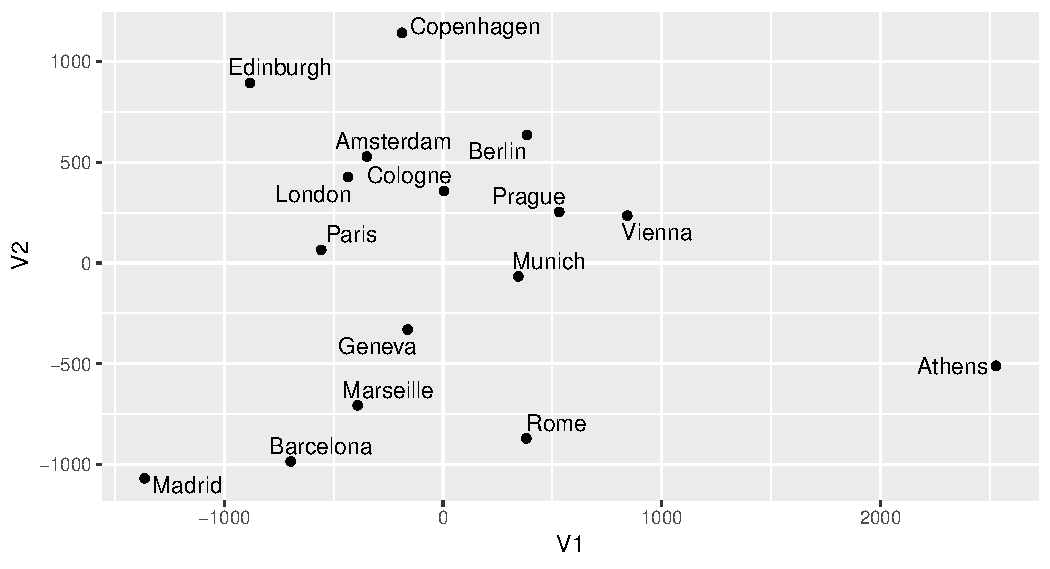
\includegraphics[width=\maxwidth]{figure/unnamed-chunk-10-1} 

\end{knitrout}
  
\end{frame}


\begin{frame}[fragile]{Comments}
  
  \begin{itemize}
  \item North-south not quite right: Edinburgh and Copenhagen on same
    latitude, also Amsterdam and Berlin; Athens should be south of Rome.
  \item Rotating clockwise by about 45 degrees should fix that.
  \item General point: MDS only uses distances, so answer can be
    ``off'' by rotation (as here) or reflection (flipping over, say
    exchanging west and east while leaving north and south same). 
  \end{itemize} 
  
\end{frame}

\begin{frame}[fragile]{Exploring the map by plotting in 3 dimensions}
  
  \begin{itemize}
  \item Package \texttt{rgl} makes 3D plots.
  \item We have to fake up a 3rd dimension (by setting all its values
    to 1).
  \item Try this code:
\begin{knitrout}
\definecolor{shadecolor}{rgb}{0.969, 0.969, 0.969}\color{fgcolor}\begin{kframe}
\begin{alltt}
\hlkwd{library}\hlstd{(rgl)}
\hlstd{es.2}\hlkwb{=}\hlkwd{cbind}\hlstd{(europe.scale,}\hlnum{1}\hlstd{)}
\hlkwd{plot3d}\hlstd{(es.2,}\hlkwc{zlim}\hlstd{=}\hlkwd{c}\hlstd{(}\hlopt{-}\hlnum{1000}\hlstd{,}\hlnum{1000}\hlstd{))}
\hlkwd{text3d}\hlstd{(es.2,}\hlkwc{text}\hlstd{=d}\hlopt{$}\hlstd{city)}
\end{alltt}
\end{kframe}
\end{knitrout}
\item Opens a graphics window with the cities plotted and named.
\item Click and hold left mouse button to rotate plot. ``Rotate away''
  3rd dimension to get a possible map (that preserves distances). 
  \end{itemize}
  
\end{frame}


\begin{frame}[fragile]{Ontario, the same way}
  
\begin{knitrout}
\definecolor{shadecolor}{rgb}{0.969, 0.969, 0.969}\color{fgcolor}\begin{kframe}
\begin{alltt}
\hlstd{ontario}\hlkwb{=}\hlkwd{read.csv}\hlstd{(}\hlstr{"ontario-road-distances.csv"}\hlstd{,}\hlkwc{header}\hlstd{=T)}
\hlstd{ontario.d}\hlkwb{=}\hlkwd{as.dist}\hlstd{(ontario)}
\hlstd{ontario.scale}\hlkwb{=}\hlkwd{cmdscale}\hlstd{(ontario.d)}
\hlstd{d}\hlkwb{=}\hlkwd{data.frame}\hlstd{(ontario.scale,}\hlkwc{city}\hlstd{=}\hlkwd{colnames}\hlstd{(ontario))}
\hlstd{g}\hlkwb{=}\hlkwd{ggplot}\hlstd{(d,}\hlkwd{aes}\hlstd{(}\hlkwc{x}\hlstd{=X1,}\hlkwc{y}\hlstd{=X2,}\hlkwc{label}\hlstd{=city))}\hlopt{+}
  \hlkwd{geom_point}\hlstd{()}\hlopt{+}\hlkwd{coord_fixed}\hlstd{()}\hlopt{+}
  \hlkwd{geom_text_repel}\hlstd{()}
\end{alltt}
\end{kframe}
\end{knitrout}

  
\end{frame}

\begin{frame}[fragile]{The plot}
  
\begin{knitrout}
\definecolor{shadecolor}{rgb}{0.969, 0.969, 0.969}\color{fgcolor}
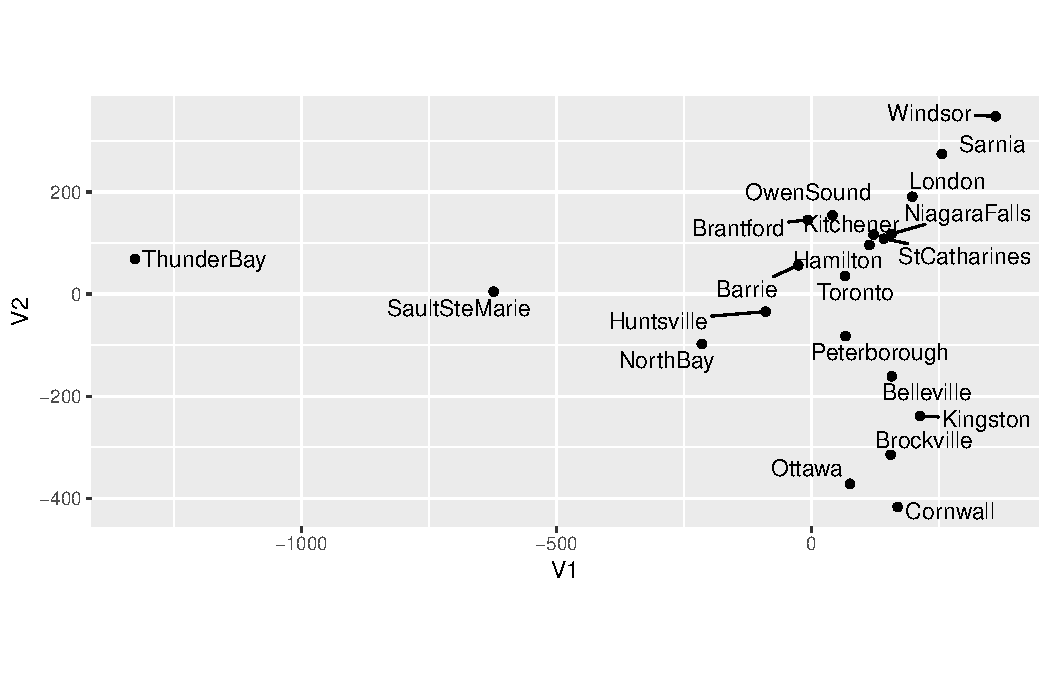
\includegraphics[width=\maxwidth]{figure/flimby-1} 

\end{knitrout}
  
  
\end{frame}

\begin{frame}[fragile]{Comments}
  
  \begin{itemize}
  \item Plot dominated by Thunder Bay and Sault Ste Marie (so distant
    from everything else).
  \item Remove and try again:

\begin{knitrout}\footnotesize
\definecolor{shadecolor}{rgb}{0.969, 0.969, 0.969}\color{fgcolor}\begin{kframe}
\begin{alltt}
\hlstd{d}\hlopt{$}\hlstd{city}
\end{alltt}
\begin{verbatim}
##  [1] Barrie        Belleville    Brantford     Brockville    Cornwall     
##  [6] Hamilton      Huntsville    Kingston      Kitchener     London       
## [11] NiagaraFalls  NorthBay      Ottawa        OwenSound     Peterborough 
## [16] Sarnia        SaultSteMarie StCatharines  ThunderBay    Toronto      
## [21] Windsor      
## 21 Levels: Barrie Belleville Brantford Brockville Cornwall ... Windsor
\end{verbatim}
\end{kframe}
\end{knitrout}
%$ %$ %$

\item Cities 17 and 19 are the ones to go:
  
\begin{knitrout}\small
\definecolor{shadecolor}{rgb}{0.969, 0.969, 0.969}\color{fgcolor}\begin{kframe}
\begin{alltt}
\hlstd{ontario2}\hlkwb{=}\hlstd{ontario[}\hlkwd{c}\hlstd{(}\hlopt{-}\hlnum{17}\hlstd{,}\hlopt{-}\hlnum{19}\hlstd{),}\hlkwd{c}\hlstd{(}\hlopt{-}\hlnum{17}\hlstd{,}\hlopt{-}\hlnum{19}\hlstd{)]}
\hlstd{ontario2.d}\hlkwb{=}\hlkwd{as.dist}\hlstd{(ontario2)}
\hlstd{ontario2.scale}\hlkwb{=}\hlkwd{cmdscale}\hlstd{(ontario2.d)}
\hlstd{d2}\hlkwb{=}\hlkwd{data.frame}\hlstd{(ontario2.scale,}\hlkwc{city}\hlstd{=}\hlkwd{colnames}\hlstd{(ontario2))}
\hlstd{g2}\hlkwb{=}\hlkwd{ggplot}\hlstd{(d2,}\hlkwd{aes}\hlstd{(}\hlkwc{x}\hlstd{=X1,}\hlkwc{y}\hlstd{=X2,}\hlkwc{label}\hlstd{=city))}\hlopt{+}\hlkwd{geom_point}\hlstd{()}\hlopt{+}
  \hlkwd{coord_fixed}\hlstd{()}\hlopt{+}\hlkwd{geom_text_repel}\hlstd{()}
\end{alltt}
\end{kframe}
\end{knitrout}
      

\item Does plot look better?
  \end{itemize}
  
\end{frame}

\begin{frame}[fragile]{Plot of \texttt{ontario2.scale}}

\begin{knitrout}
\definecolor{shadecolor}{rgb}{0.969, 0.969, 0.969}\color{fgcolor}\begin{kframe}
\begin{alltt}
\hlstd{g2}
\end{alltt}
\end{kframe}
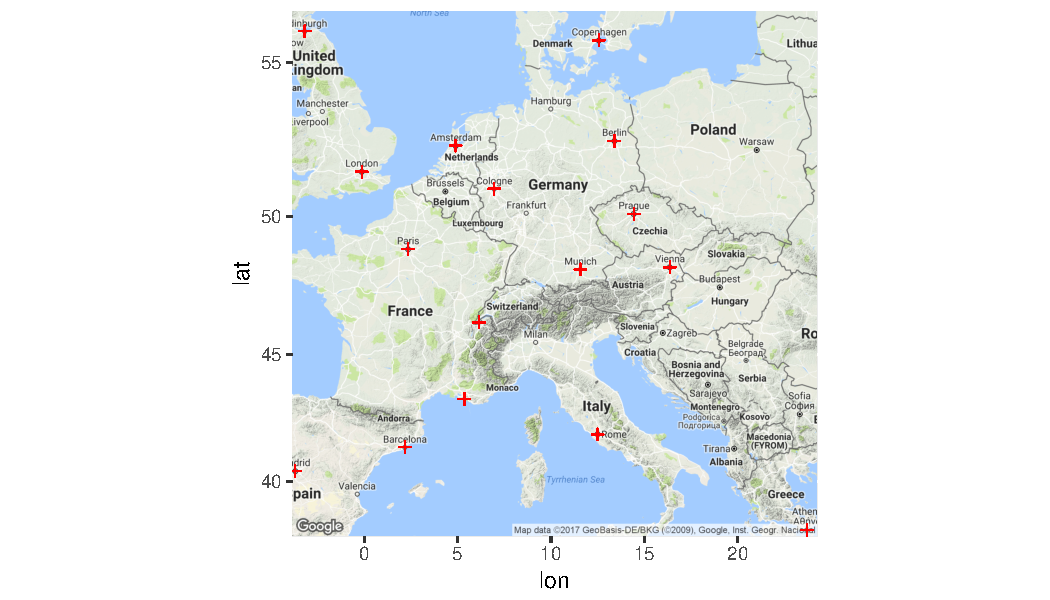
\includegraphics[width=\maxwidth]{figure/onnnscale-1} 

\end{knitrout}
  
   
\end{frame}

\begin{frame}[fragile]{What about that cluster of points?}

  \begin{itemize}
  \item Plot looks generally good, but what about that cluster of points?
  \item ``Zoom in'' on area between $-150$ and $-100$ on $x$ axis, $-50$ to 0 on
$y$ axis.
\item Code below overrides the \texttt{coord\_fixed} we had before.
  \end{itemize}


\begin{knitrout}
\definecolor{shadecolor}{rgb}{0.969, 0.969, 0.969}\color{fgcolor}\begin{kframe}
\begin{alltt}
\hlstd{g3}\hlkwb{=}\hlstd{g2}\hlopt{+}\hlkwd{coord_fixed}\hlstd{(}\hlkwc{xlim}\hlstd{=}\hlkwd{c}\hlstd{(}\hlopt{-}\hlnum{150}\hlstd{,}\hlopt{-}\hlnum{100}\hlstd{),}\hlkwc{ylim}\hlstd{=}\hlkwd{c}\hlstd{(}\hlopt{-}\hlnum{50}\hlstd{,}\hlnum{0}\hlstd{))}
\end{alltt}
\end{kframe}
\end{knitrout}

  
\end{frame}

\begin{frame}[fragile]{Zoomed-in plot}
 
Ignore the arrows to points off the map:

\begin{knitrout}
\definecolor{shadecolor}{rgb}{0.969, 0.969, 0.969}\color{fgcolor}\begin{kframe}
\begin{alltt}
\hlstd{g3}
\end{alltt}
\end{kframe}
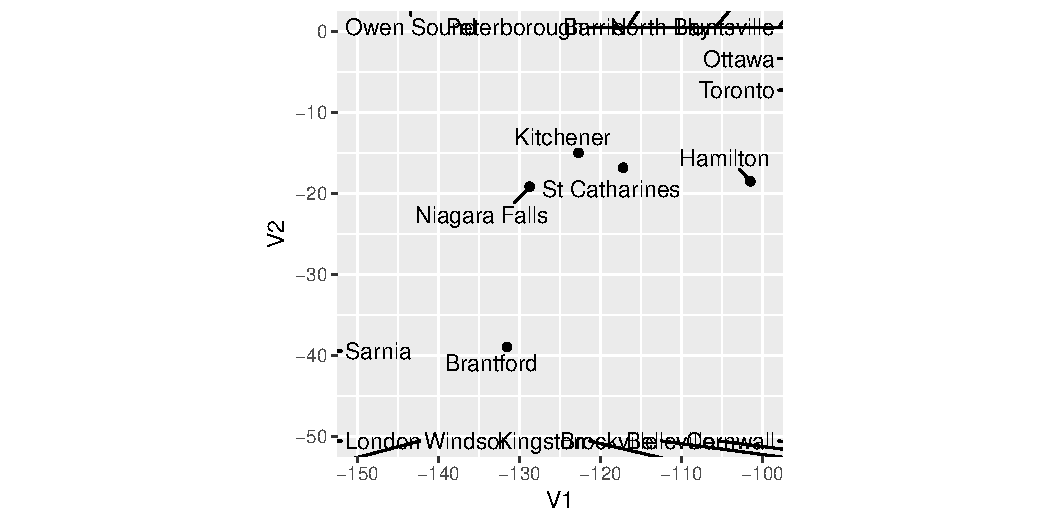
\includegraphics[width=\maxwidth]{figure/spal-1} 

\end{knitrout}

  St Catharines and Niagara Falls are nowhere near Kitchener!

  
  
\end{frame}



\begin{frame}[fragile]{Quality of fit}
  
  Calling \texttt{cmdscale} with \texttt{eig=T} gives more info:

  {\footnotesize
\begin{knitrout}
\definecolor{shadecolor}{rgb}{0.969, 0.969, 0.969}\color{fgcolor}\begin{kframe}
\begin{alltt}
\hlstd{ontario2a}\hlkwb{=}\hlkwd{cmdscale}\hlstd{(ontario2,}\hlkwc{eig}\hlstd{=T)}
\hlkwd{names}\hlstd{(ontario2a)}
\end{alltt}
\begin{verbatim}
## [1] "points" "eig"    "x"      "ac"     "GOF"
\end{verbatim}
\begin{alltt}
\hlstd{ontario2a}\hlopt{$}\hlstd{GOF}
\end{alltt}
\begin{verbatim}
## [1] 0.8381590 0.8914059
\end{verbatim}
\begin{alltt}
\hlkwd{cmdscale}\hlstd{(ontario2,}\hlnum{3}\hlstd{,}\hlkwc{eig}\hlstd{=T)}\hlopt{$}\hlstd{GOF}
\end{alltt}
\begin{verbatim}
## [1] 0.8852559 0.9414948
\end{verbatim}
\end{kframe}
\end{knitrout}
}

\begin{itemize}
\item Coordinates now in \texttt{points}.
\item \texttt{GOF} is R-squared-like measure saying how well map
  distances match real ones. Higher is better.
\item For Ontario road distances, \texttt{GOF} better for 3 dimensions
  than 2, presumably to accommodate St Catharines and Niagara Falls?
\end{itemize}
  
\end{frame}


\begin{frame}[fragile]{3-dimensional coordinates}
  
{\scriptsize
\begin{knitrout}
\definecolor{shadecolor}{rgb}{0.969, 0.969, 0.969}\color{fgcolor}\begin{kframe}
\begin{alltt}
\hlstd{ontario.3}\hlkwb{=}\hlkwd{cmdscale}\hlstd{(ontario2.d,}\hlnum{3}\hlstd{)}
\hlstd{ontario.3}
\end{alltt}
\begin{verbatim}
##                    [,1]         [,2]       [,3]
## Barrie        -38.70111  121.9167146   4.168684
## Belleville    145.74321  -82.8359816   1.526172
## Brantford    -131.51866  -38.9277965  14.085047
## Brockville    298.02697 -105.6039755  -7.738994
## Cornwall      397.22871 -103.6445206 -21.977485
## Hamilton     -101.47284  -18.4865757  30.049990
## Huntsville     62.41456  197.9151274 -14.049037
## Kingston      214.41469 -129.3939106  10.785262
## Kitchener    -122.68957  -14.9820650  -6.443508
## London       -207.75236  -51.6295564 -36.541619
## NiagaraFalls -128.72171  -19.1486968 155.149360
## NorthBay      145.73913  299.8542830 -25.424334
## Ottawa        367.87357   -4.3010846 -47.177760
## OwenSound    -144.82323  125.3036987 -16.023323
## Peterborough   82.53780    0.5508137  -6.924234
## Sarnia       -298.69291  -39.4332816 -72.458986
## StCatharines -117.19167  -16.7948120 122.628327
## Toronto       -34.25551   -4.7492448  15.843422
## Windsor      -388.15907 -115.6091356 -99.476983
\end{verbatim}
\end{kframe}
\end{knitrout}
}
  
\end{frame}

\begin{frame}[fragile]{RGL code for 3 dimensions}
  
\begin{knitrout}
\definecolor{shadecolor}{rgb}{0.969, 0.969, 0.969}\color{fgcolor}\begin{kframe}
\begin{alltt}
\hlkwd{library}\hlstd{(rgl)}
\hlkwd{plot3d}\hlstd{(ontario.3)}
\hlkwd{text3d}\hlstd{(ontario.3,}\hlkwc{text}\hlstd{=d2}\hlopt{$}\hlstd{city)}
\end{alltt}
\end{kframe}
\end{knitrout}



\end{frame}

\begin{frame}[fragile]{Comparing MDS solution with ``reality'':
    Procrustes rotation}
  
  \begin{itemize}
  \item How to tell that an MDS map makes a good correspondence with ``what
    should be''?
  \item Problem: MDS map might be rotated/scaled/reflected from reality.
  \item How to find rotation/scaling/reflection that best matches reality?
  \item Answer: \textbf{Procrustes rotation}.
  \item In R: \texttt{procOPA} in package \texttt{shapes}.
  \end{itemize}
  
\end{frame}

\begin{frame}[fragile]{``True'' coordinates}

  \begin{itemize}
  \item Get latitudes and longitudes of cities by geocoding, as
    before. Glue ``ON'' onto city names to make sure we get right ones:
    
\begin{knitrout}\small
\definecolor{shadecolor}{rgb}{0.969, 0.969, 0.969}\color{fgcolor}\begin{kframe}
\begin{alltt}
\hlstd{lookup}\hlkwb{=}\hlkwd{paste}\hlstd{(d2}\hlopt{$}\hlstd{city,}\hlstr{"ON"}\hlstd{)}
\hlstd{latlong}\hlkwb{=}\hlkwd{geocode}\hlstd{(lookup)}
\end{alltt}


{\ttfamily\noindent\color{warningcolor}{\#\# Warning in readLines(connect, warn = FALSE): URL 'https://maps.googleapis.com/maps/api/geocode/json?address=Barrie\%20ON': status was 'Couldn't resolve host name'}}

{\ttfamily\noindent\color{warningcolor}{\#\# Warning in FUN(X[[i]], ...):\ \  geocoding failed for "{}Barrie ON"{}.\\\#\#\ \  if accompanied by 500 Internal Server Error with using dsk, try google.}}

{\ttfamily\noindent\color{warningcolor}{\#\# Warning in readLines(connect, warn = FALSE): URL 'https://maps.googleapis.com/maps/api/geocode/json?address=Belleville\%20ON': status was 'Couldn't resolve host name'}}

{\ttfamily\noindent\color{warningcolor}{\#\# Warning in FUN(X[[i]], ...):\ \  geocoding failed for "{}Belleville ON"{}.\\\#\#\ \  if accompanied by 500 Internal Server Error with using dsk, try google.}}

{\ttfamily\noindent\color{warningcolor}{\#\# Warning in readLines(connect, warn = FALSE): URL 'https://maps.googleapis.com/maps/api/geocode/json?address=Brantford\%20ON': status was 'Couldn't resolve host name'}}

{\ttfamily\noindent\color{warningcolor}{\#\# Warning in FUN(X[[i]], ...):\ \  geocoding failed for "{}Brantford ON"{}.\\\#\#\ \  if accompanied by 500 Internal Server Error with using dsk, try google.}}

{\ttfamily\noindent\color{warningcolor}{\#\# Warning in readLines(connect, warn = FALSE): URL 'https://maps.googleapis.com/maps/api/geocode/json?address=Brockville\%20ON': status was 'Couldn't resolve host name'}}

{\ttfamily\noindent\color{warningcolor}{\#\# Warning in FUN(X[[i]], ...):\ \  geocoding failed for "{}Brockville ON"{}.\\\#\#\ \  if accompanied by 500 Internal Server Error with using dsk, try google.}}

{\ttfamily\noindent\color{warningcolor}{\#\# Warning in readLines(connect, warn = FALSE): URL 'https://maps.googleapis.com/maps/api/geocode/json?address=Cornwall\%20ON': status was 'Couldn't resolve host name'}}

{\ttfamily\noindent\color{warningcolor}{\#\# Warning in FUN(X[[i]], ...):\ \  geocoding failed for "{}Cornwall ON"{}.\\\#\#\ \  if accompanied by 500 Internal Server Error with using dsk, try google.}}

{\ttfamily\noindent\color{warningcolor}{\#\# Warning in readLines(connect, warn = FALSE): URL 'https://maps.googleapis.com/maps/api/geocode/json?address=Hamilton\%20ON': status was 'Couldn't resolve host name'}}

{\ttfamily\noindent\color{warningcolor}{\#\# Warning in FUN(X[[i]], ...):\ \  geocoding failed for "{}Hamilton ON"{}.\\\#\#\ \  if accompanied by 500 Internal Server Error with using dsk, try google.}}

{\ttfamily\noindent\color{warningcolor}{\#\# Warning in readLines(connect, warn = FALSE): URL 'https://maps.googleapis.com/maps/api/geocode/json?address=Huntsville\%20ON': status was 'Couldn't resolve host name'}}

{\ttfamily\noindent\color{warningcolor}{\#\# Warning in FUN(X[[i]], ...):\ \  geocoding failed for "{}Huntsville ON"{}.\\\#\#\ \  if accompanied by 500 Internal Server Error with using dsk, try google.}}

{\ttfamily\noindent\color{warningcolor}{\#\# Warning in readLines(connect, warn = FALSE): URL 'https://maps.googleapis.com/maps/api/geocode/json?address=Kingston\%20ON': status was 'Couldn't resolve host name'}}

{\ttfamily\noindent\color{warningcolor}{\#\# Warning in FUN(X[[i]], ...):\ \  geocoding failed for "{}Kingston ON"{}.\\\#\#\ \  if accompanied by 500 Internal Server Error with using dsk, try google.}}

{\ttfamily\noindent\color{warningcolor}{\#\# Warning in readLines(connect, warn = FALSE): URL 'https://maps.googleapis.com/maps/api/geocode/json?address=Kitchener\%20ON': status was 'Couldn't resolve host name'}}

{\ttfamily\noindent\color{warningcolor}{\#\# Warning in FUN(X[[i]], ...):\ \  geocoding failed for "{}Kitchener ON"{}.\\\#\#\ \  if accompanied by 500 Internal Server Error with using dsk, try google.}}

{\ttfamily\noindent\color{warningcolor}{\#\# Warning in readLines(connect, warn = FALSE): URL 'https://maps.googleapis.com/maps/api/geocode/json?address=London\%20ON': status was 'Couldn't resolve host name'}}

{\ttfamily\noindent\color{warningcolor}{\#\# Warning in FUN(X[[i]], ...):\ \  geocoding failed for "{}London ON"{}.\\\#\#\ \  if accompanied by 500 Internal Server Error with using dsk, try google.}}

{\ttfamily\noindent\color{warningcolor}{\#\# Warning in readLines(connect, warn = FALSE): URL 'https://maps.googleapis.com/maps/api/geocode/json?address=NiagaraFalls\%20ON': status was 'Couldn't resolve host name'}}

{\ttfamily\noindent\color{warningcolor}{\#\# Warning in FUN(X[[i]], ...):\ \  geocoding failed for "{}NiagaraFalls ON"{}.\\\#\#\ \  if accompanied by 500 Internal Server Error with using dsk, try google.}}

{\ttfamily\noindent\color{warningcolor}{\#\# Warning in readLines(connect, warn = FALSE): URL 'https://maps.googleapis.com/maps/api/geocode/json?address=NorthBay\%20ON': status was 'Couldn't resolve host name'}}

{\ttfamily\noindent\color{warningcolor}{\#\# Warning in FUN(X[[i]], ...):\ \  geocoding failed for "{}NorthBay ON"{}.\\\#\#\ \  if accompanied by 500 Internal Server Error with using dsk, try google.}}

{\ttfamily\noindent\color{warningcolor}{\#\# Warning in readLines(connect, warn = FALSE): URL 'https://maps.googleapis.com/maps/api/geocode/json?address=Ottawa\%20ON': status was 'Couldn't resolve host name'}}

{\ttfamily\noindent\color{warningcolor}{\#\# Warning in FUN(X[[i]], ...):\ \  geocoding failed for "{}Ottawa ON"{}.\\\#\#\ \  if accompanied by 500 Internal Server Error with using dsk, try google.}}

{\ttfamily\noindent\color{warningcolor}{\#\# Warning in readLines(connect, warn = FALSE): URL 'https://maps.googleapis.com/maps/api/geocode/json?address=OwenSound\%20ON': status was 'Couldn't resolve host name'}}

{\ttfamily\noindent\color{warningcolor}{\#\# Warning in FUN(X[[i]], ...):\ \  geocoding failed for "{}OwenSound ON"{}.\\\#\#\ \  if accompanied by 500 Internal Server Error with using dsk, try google.}}

{\ttfamily\noindent\color{warningcolor}{\#\# Warning in readLines(connect, warn = FALSE): URL 'https://maps.googleapis.com/maps/api/geocode/json?address=Peterborough\%20ON': status was 'Couldn't resolve host name'}}

{\ttfamily\noindent\color{warningcolor}{\#\# Warning in FUN(X[[i]], ...):\ \  geocoding failed for "{}Peterborough ON"{}.\\\#\#\ \  if accompanied by 500 Internal Server Error with using dsk, try google.}}

{\ttfamily\noindent\color{warningcolor}{\#\# Warning in readLines(connect, warn = FALSE): URL 'https://maps.googleapis.com/maps/api/geocode/json?address=Sarnia\%20ON': status was 'Couldn't resolve host name'}}

{\ttfamily\noindent\color{warningcolor}{\#\# Warning in FUN(X[[i]], ...):\ \  geocoding failed for "{}Sarnia ON"{}.\\\#\#\ \  if accompanied by 500 Internal Server Error with using dsk, try google.}}

{\ttfamily\noindent\color{warningcolor}{\#\# Warning in readLines(connect, warn = FALSE): URL 'https://maps.googleapis.com/maps/api/geocode/json?address=StCatharines\%20ON': status was 'Couldn't resolve host name'}}

{\ttfamily\noindent\color{warningcolor}{\#\# Warning in FUN(X[[i]], ...):\ \  geocoding failed for "{}StCatharines ON"{}.\\\#\#\ \  if accompanied by 500 Internal Server Error with using dsk, try google.}}

{\ttfamily\noindent\color{warningcolor}{\#\# Warning in readLines(connect, warn = FALSE): URL 'https://maps.googleapis.com/maps/api/geocode/json?address=Toronto\%20ON': status was 'Couldn't resolve host name'}}

{\ttfamily\noindent\color{warningcolor}{\#\# Warning in FUN(X[[i]], ...):\ \  geocoding failed for "{}Toronto ON"{}.\\\#\#\ \  if accompanied by 500 Internal Server Error with using dsk, try google.}}

{\ttfamily\noindent\color{warningcolor}{\#\# Warning in readLines(connect, warn = FALSE): URL 'https://maps.googleapis.com/maps/api/geocode/json?address=Windsor\%20ON': status was 'Couldn't resolve host name'}}

{\ttfamily\noindent\color{warningcolor}{\#\# Warning in FUN(X[[i]], ...):\ \  geocoding failed for "{}Windsor ON"{}.\\\#\#\ \  if accompanied by 500 Internal Server Error with using dsk, try google.}}\begin{alltt}
\hlkwd{head}\hlstd{(latlong)}
\end{alltt}
\begin{verbatim}
##   lon lat
## 1  NA  NA
## 2  NA  NA
## 3  NA  NA
## 4  NA  NA
## 5  NA  NA
## 6  NA  NA
\end{verbatim}
\end{kframe}
\end{knitrout}

  \item Not $(x,y)$ coordinates: one degree of latitude is always
    110.25 km, but one degree of longitude is only that at the equator
    (less than that as you move further north, down to 0 km at north
    pole).
  \item Make coordinates by multiplying by cosine of ``typical'' latitude.
  \end{itemize}
  
\end{frame}

\begin{frame}[fragile]{``True'' coordinates part 2}
  
  \begin{itemize}
  \item Find mean latitude:
\begin{knitrout}
\definecolor{shadecolor}{rgb}{0.969, 0.969, 0.969}\color{fgcolor}\begin{kframe}
\begin{alltt}
\hlstd{m}\hlkwb{=}\hlkwd{mean}\hlstd{(latlong}\hlopt{$}\hlstd{lat); m}
\end{alltt}
\begin{verbatim}
## [1] NA
\end{verbatim}
\end{kframe}
\end{knitrout}

\item Turn into radians and find its cosine:
  
\begin{knitrout}
\definecolor{shadecolor}{rgb}{0.969, 0.969, 0.969}\color{fgcolor}\begin{kframe}
\begin{alltt}
\hlstd{mult}\hlkwb{=}\hlkwd{cos}\hlstd{(m}\hlopt{*}\hlstd{pi}\hlopt{/}\hlnum{180}\hlstd{); mult}
\end{alltt}
\begin{verbatim}
## [1] NA
\end{verbatim}
\end{kframe}
\end{knitrout}

\item Create ``true'' coords by multiplying the longitudes by
  that. This needs to be R \texttt{matrix}, not data frame:
  
\begin{knitrout}\footnotesize
\definecolor{shadecolor}{rgb}{0.969, 0.969, 0.969}\color{fgcolor}\begin{kframe}
\begin{alltt}
\hlstd{truecoord}\hlkwb{=}\hlkwd{with}\hlstd{(latlong,}\hlkwd{cbind}\hlstd{(}\hlkwc{x}\hlstd{=lon}\hlopt{*}\hlstd{mult,}\hlkwc{y}\hlstd{=lat))}
\hlkwd{head}\hlstd{(truecoord)}
\end{alltt}
\begin{verbatim}
##       x  y
## [1,] NA NA
## [2,] NA NA
## [3,] NA NA
## [4,] NA NA
## [5,] NA NA
## [6,] NA NA
\end{verbatim}
\end{kframe}
\end{knitrout}
  \end{itemize}
  
\end{frame}

\begin{frame}[fragile]{Using \texttt{procOPA}}

  \begin{itemize}
  \item Feed 2 things into \texttt{procOPA}: first, ``true''
    coordinates, second MDS coordinates.
  \item Get out: 
    \begin{itemize}
    \item     (centred and scaled) first set of coordinates \texttt{Ahat}
    \item (centred and scaled) second set of coordinates \texttt{Bhat}
    \item sum of squared differences between two sets of coordinates \texttt{OSS}
      \item Rotation matrix \texttt{R}
    \end{itemize}
    
\begin{knitrout}
\definecolor{shadecolor}{rgb}{0.969, 0.969, 0.969}\color{fgcolor}\begin{kframe}
\begin{alltt}
\hlkwd{suppressMessages}\hlstd{(}\hlkwd{library}\hlstd{(shapes))}
\hlstd{ontario.pro}\hlkwb{=}\hlkwd{procOPA}\hlstd{(truecoord,ontario2.scale)}
\end{alltt}


{\ttfamily\noindent\bfseries\color{errorcolor}{\#\# Error in svd(x): infinite or missing values in 'x'}}\end{kframe}
\end{knitrout}

\item Make a data frame to plot with, stacking $x$ and $y$ (that's
  what \texttt{ggplot} likes):
\begin{knitrout}\small
\definecolor{shadecolor}{rgb}{0.969, 0.969, 0.969}\color{fgcolor}\begin{kframe}
\begin{alltt}
\hlstd{ncity}\hlkwb{=}\hlkwd{length}\hlstd{(d2}\hlopt{$}\hlstd{city)}
\hlstd{dp}\hlkwb{=}\hlkwd{with}\hlstd{(ontario.pro,}\hlkwd{data.frame}\hlstd{(}\hlkwc{x}\hlstd{=}\hlkwd{c}\hlstd{(Ahat[,}\hlnum{1}\hlstd{],Bhat[,}\hlnum{1}\hlstd{]),}
  \hlkwc{y}\hlstd{=}\hlkwd{c}\hlstd{(Ahat[,}\hlnum{2}\hlstd{],Bhat[,}\hlnum{2}\hlstd{]),}\hlkwc{which}\hlstd{=}\hlkwd{c}\hlstd{(}\hlkwd{rep}\hlstd{(}\hlstr{"actual"}\hlstd{,ncity),}\hlkwd{rep}\hlstd{(}\hlstr{"MDS"}\hlstd{,ncity)),}
  \hlkwc{city}\hlstd{=}\hlkwd{rep}\hlstd{(d2}\hlopt{$}\hlstd{city,}\hlnum{2}\hlstd{)))}
\end{alltt}


{\ttfamily\noindent\bfseries\color{errorcolor}{\#\# Error in with(ontario.pro, data.frame(x = c(Ahat[, 1], Bhat[, 1]), y = c(Ahat[, : object 'ontario.pro' not found}}\begin{alltt}
\hlkwd{names}\hlstd{(dp)}
\end{alltt}


{\ttfamily\noindent\bfseries\color{errorcolor}{\#\# Error in eval(expr, envir, enclos): object 'dp' not found}}\end{kframe}
\end{knitrout}

  \end{itemize}
  
\end{frame}

\begin{frame}[fragile]{Procrustes rotation plot}
  
  \begin{itemize}
  \item Strategy: plot all the locations, and colour them by whether
    they were the true location (red) or the MDS one (blue), which is
    in \texttt{which}. Label each location with the city name in the
    appropriate colour.
  \item I realized it
    was actually easy to join the two instances of a city by a line
    (in green, here, 3rd line) by setting \texttt{group=city}:
\begin{knitrout}
\definecolor{shadecolor}{rgb}{0.969, 0.969, 0.969}\color{fgcolor}\begin{kframe}
\begin{alltt}
\hlstd{g}\hlkwb{=}\hlkwd{ggplot}\hlstd{(dp,}\hlkwd{aes}\hlstd{(}\hlkwc{x}\hlstd{=x,}\hlkwc{y}\hlstd{=y,}\hlkwc{colour}\hlstd{=which,}\hlkwc{label}\hlstd{=city))}\hlopt{+}
  \hlkwd{geom_point}\hlstd{()}\hlopt{+}
  \hlkwd{geom_line}\hlstd{(}\hlkwd{aes}\hlstd{(}\hlkwc{group}\hlstd{=city),}\hlkwc{colour}\hlstd{=}\hlstr{"green"}\hlstd{)}\hlopt{+}
  \hlkwd{geom_text_repel}\hlstd{()}
\end{alltt}


{\ttfamily\noindent\bfseries\color{errorcolor}{\#\# Error in ggplot(dp, aes(x = x, y = y, colour = which, label = city)): object 'dp' not found}}\end{kframe}
\end{knitrout}
\item On plot, look to see whether points that are same city are
  joined by a short green line (good) or a long one (bad).
  \end{itemize}
\end{frame}

\begin{frame}{The maps}
 
\begin{knitrout}
\definecolor{shadecolor}{rgb}{0.969, 0.969, 0.969}\color{fgcolor}
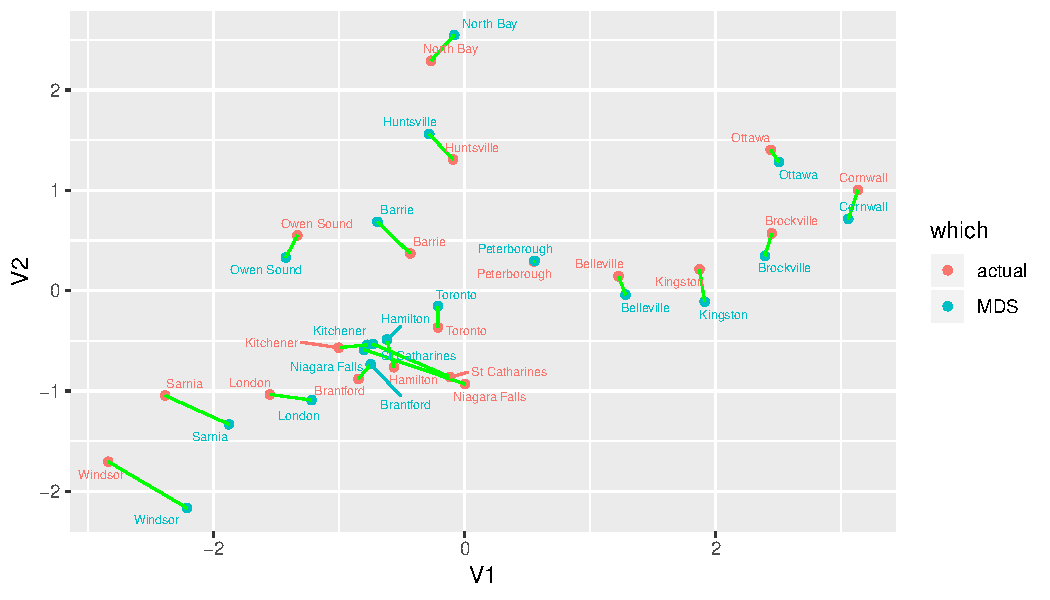
\includegraphics[width=\maxwidth]{figure/prosesto-1} 

\end{knitrout}
  
  
%  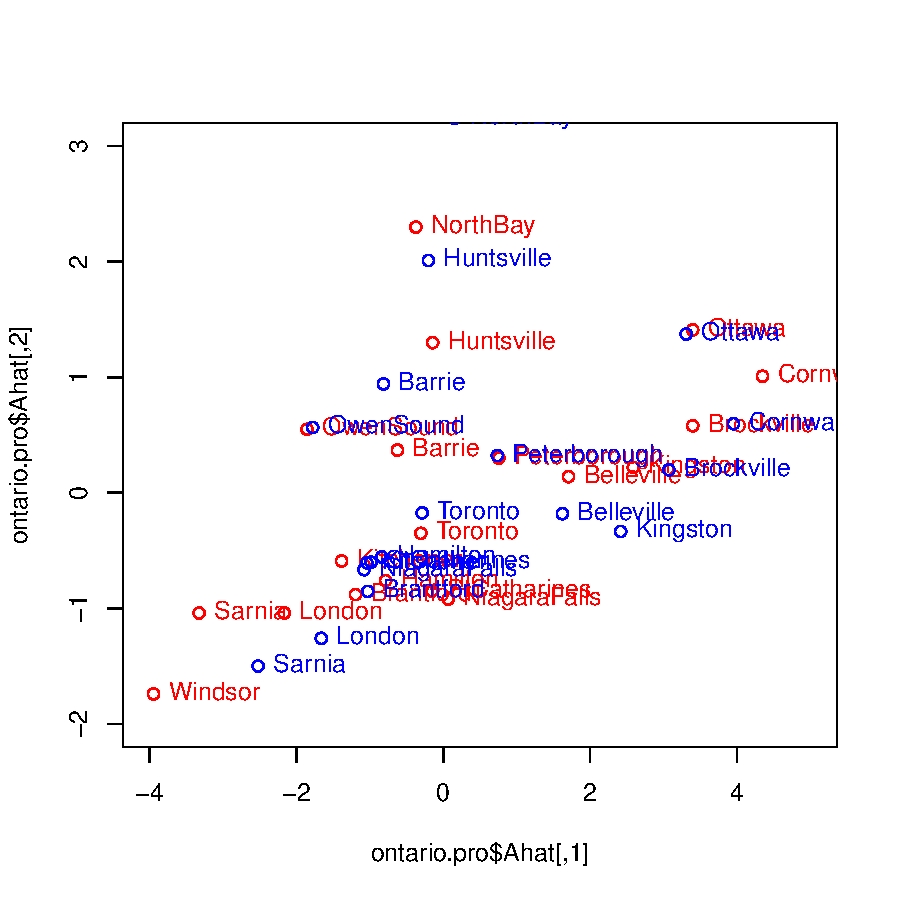
\includegraphics[height=\textheight]{bMDS-ont-proc}
  
\end{frame}

\begin{frame}[fragile]{Comments}
  
  \begin{itemize}
  \item True locations red, MDS locations blue
  \item Most things in roughly right place (esp.\ relative to other things)
  \item Extreme cities off by a bit, but OK relative to neighbours.
  \item St Catharines, Niagara Falls off by most.
  \end{itemize}
  
\end{frame}

\begin{frame}[fragile]{Rotation matrix}
  
  Shows how MDS map needs to be rotated to get best match with actual coordinates:
  
\begin{knitrout}
\definecolor{shadecolor}{rgb}{0.969, 0.969, 0.969}\color{fgcolor}\begin{kframe}
\begin{alltt}
\hlstd{ontario.pro}\hlopt{$}\hlstd{R}
\end{alltt}


{\ttfamily\noindent\bfseries\color{errorcolor}{\#\# Error in eval(expr, envir, enclos): object 'ontario.pro' not found}}\end{kframe}
\end{knitrout}

Rotation angle $\theta$ such that $\cos\theta=0.885$,
$\sin\theta=0.466$: $\theta=23$ degrees (counterclockwise). 
%$ %$ %$
  
\end{frame}

\begin{frame}[fragile]{Is that right? Look at MDS map again}
  
\begin{knitrout}
\definecolor{shadecolor}{rgb}{0.969, 0.969, 0.969}\color{fgcolor}\begin{kframe}
\begin{alltt}
\hlstd{g2}
\end{alltt}
\end{kframe}
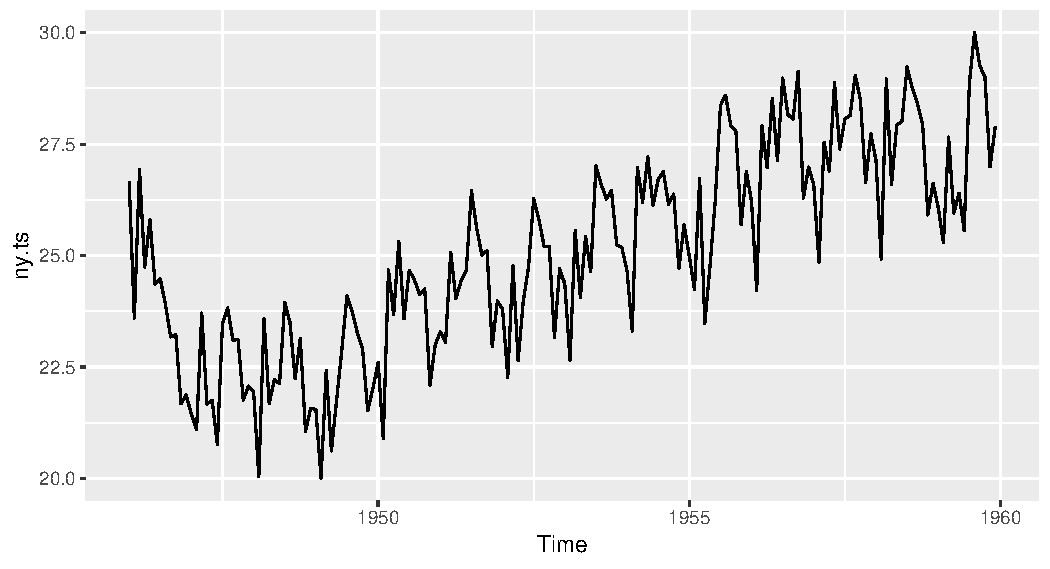
\includegraphics[width=\maxwidth]{figure/unnamed-chunk-25-1} 

\end{knitrout}

23 degrees counterclockwise seems about right.
  
\end{frame}

\begin{frame}[fragile]{A cube}
  
  
\begin{verbatim}
  a-----b
  |\    |\
  | c---- d
  | |   | |
  e-|---f |
   \|    \|
    g-----h
\end{verbatim}

Cube has side length 1, so distance across diagonal on same face is $\sqrt{2}\simeq 1.4$ and ``long'' diagonal of cube is $\sqrt{3}\simeq 1.7$. 
  
\vspace{3ex}

Try MDS on this obviously 3-dimensional data.

\end{frame}

\begin{frame}[fragile]{Cube data as distances}
 
\begin{knitrout}
\definecolor{shadecolor}{rgb}{0.969, 0.969, 0.969}\color{fgcolor}\begin{kframe}
\begin{alltt}
\hlstd{cube}\hlkwb{=}\hlkwd{read.table}\hlstd{(}\hlstr{"cube.txt"}\hlstd{,}\hlkwc{header}\hlstd{=T)}
\hlstd{cube}
\end{alltt}
\begin{verbatim}
##     a   b   c   d   e   f  g  h
## a 0.0  NA  NA  NA  NA  NA NA NA
## b 1.0 0.0  NA  NA  NA  NA NA NA
## c 1.0 1.0 0.0  NA  NA  NA NA NA
## d 1.4 1.0 1.0 0.0  NA  NA NA NA
## e 1.0 1.4 1.4 1.7 0.0  NA NA NA
## f 1.4 1.0 1.7 1.4 1.0 0.0 NA NA
## g 1.4 1.7 1.0 1.4 1.0 1.4  0 NA
## h 1.7 1.4 1.4 1.0 1.4 1.0  1  0
\end{verbatim}
\end{kframe}
\end{knitrout}
  
\end{frame}

\begin{frame}[fragile]{Making \texttt{dist} object}
  
\begin{knitrout}
\definecolor{shadecolor}{rgb}{0.969, 0.969, 0.969}\color{fgcolor}\begin{kframe}
\begin{alltt}
\hlstd{cube.d}\hlkwb{=}\hlkwd{as.dist}\hlstd{(cube)}
\hlstd{cube.d}
\end{alltt}
\begin{verbatim}
##     a   b   c   d   e   f   g
## b 1.0                        
## c 1.0 1.0                    
## d 1.4 1.0 1.0                
## e 1.0 1.4 1.4 1.7            
## f 1.4 1.0 1.7 1.4 1.0        
## g 1.4 1.7 1.0 1.4 1.0 1.4    
## h 1.7 1.4 1.4 1.0 1.4 1.0 1.0
\end{verbatim}
\end{kframe}
\end{knitrout}

\end{frame}

\begin{frame}[fragile]{MDS and plotting commands}

  \begin{itemize}
  \item   By default in 2 dimensions; save the extra stuff for later:
\begin{knitrout}
\definecolor{shadecolor}{rgb}{0.969, 0.969, 0.969}\color{fgcolor}\begin{kframe}
\begin{alltt}
\hlstd{cube.2}\hlkwb{=}\hlkwd{cmdscale}\hlstd{(cube.d,}\hlkwc{eig}\hlstd{=T)}
\end{alltt}
\end{kframe}
\end{knitrout}
\item Make data frame to plot, remembering the points to plot are in
  \texttt{points} now:
  
\begin{knitrout}
\definecolor{shadecolor}{rgb}{0.969, 0.969, 0.969}\color{fgcolor}\begin{kframe}
\begin{alltt}
\hlstd{d}\hlkwb{=}\hlkwd{data.frame}\hlstd{(cube.2}\hlopt{$}\hlstd{points,}\hlkwc{corners}\hlstd{=}\hlkwd{names}\hlstd{(cube))}
\hlkwd{names}\hlstd{(d)}
\end{alltt}
\begin{verbatim}
## [1] "X1"      "X2"      "corners"
\end{verbatim}
\end{kframe}
\end{knitrout}
\item Plot points labelled by our names for the corners:
  
\begin{knitrout}
\definecolor{shadecolor}{rgb}{0.969, 0.969, 0.969}\color{fgcolor}\begin{kframe}
\begin{alltt}
\hlstd{g}\hlkwb{=}\hlkwd{ggplot}\hlstd{(d,}\hlkwd{aes}\hlstd{(}\hlkwc{x}\hlstd{=X1,}\hlkwc{y}\hlstd{=X2,}\hlkwc{label}\hlstd{=corners))}\hlopt{+}
  \hlkwd{geom_point}\hlstd{()}\hlopt{+}\hlkwd{geom_text_repel}\hlstd{()}
\end{alltt}
\end{kframe}
\end{knitrout}
  \end{itemize}
  

\end{frame}


\begin{frame}[fragile]{The ``cube''}
 
\begin{knitrout}
\definecolor{shadecolor}{rgb}{0.969, 0.969, 0.969}\color{fgcolor}

\includegraphics[width=\maxwidth]{figure/bianconeri-1} 

\end{knitrout}

Not good.
  
  
  
\end{frame}


\begin{frame}[fragile]{2 and 3 dimensions}
  
\begin{knitrout}
\definecolor{shadecolor}{rgb}{0.969, 0.969, 0.969}\color{fgcolor}\begin{kframe}
\begin{alltt}
\hlstd{cube.3}\hlkwb{=}\hlkwd{cmdscale}\hlstd{(cube.d,}\hlnum{3}\hlstd{,}\hlkwc{eig}\hlstd{=T)}
\hlstd{cube.2}\hlopt{$}\hlstd{GOF}
\end{alltt}
\begin{verbatim}
## [1] 0.639293 0.664332
\end{verbatim}
\begin{alltt}
\hlstd{cube.3}\hlopt{$}\hlstd{GOF}
\end{alltt}
\begin{verbatim}
## [1] 0.9143532 0.9501654
\end{verbatim}
\end{kframe}
\end{knitrout}

\begin{itemize}
\item Really need 3rd dimension to represent cube.
\end{itemize}
  
\end{frame}


\begin{frame}[fragile]{Non-metric scaling}
  
  \begin{itemize}
  \item Sometimes distances not meaningful \emph{as distances}
  \item Only order matters: closest should be closest, farthest
    farthest on map, but how much further doesn't matter.
  \item Non-metric scaling, aims to minimize \textbf{stress}, measure
    of lack of fit.
  \item Example: languages. Make map based on ``similarity'' of number
    names, without requiring that 1 is ``eight times better'' than 8.
  \end{itemize}
  
\end{frame}

\begin{frame}[fragile]{The languages}

  \begin{itemize}
  \item Recall language data (from cluster analysis): 1--10, measure dissimilarity between two languages by how many number names {\em differ} in first letter:

    
\begin{knitrout}
\definecolor{shadecolor}{rgb}{0.969, 0.969, 0.969}\color{fgcolor}\begin{kframe}
\begin{alltt}
\hlstd{number.d}\hlkwb{=}\hlkwd{read.table}\hlstd{(}\hlstr{"languages.txt"}\hlstd{,}\hlkwc{header}\hlstd{=T)}
\hlstd{number.d}
\end{alltt}
\begin{verbatim}
##    en no dk nl de fr es it pl hu fi
## en  0  2  2  7  6  6  6  6  7  9  9
## no  2  0  1  5  4  6  6  6  7  8  9
## dk  2  1  0  6  5  6  5  5  6  8  9
## nl  7  5  6  0  5  9  9  9 10  8  9
## de  6  4  5  5  0  7  7  7  8  9  9
## fr  6  6  6  9  7  0  2  1  5 10  9
## es  6  6  5  9  7  2  0  1  3 10  9
## it  6  6  5  9  7  1  1  0  4 10  9
## pl  7  7  6 10  8  5  3  4  0 10  9
## hu  9  8  8  8  9 10 10 10 10  0  8
## fi  9  9  9  9  9  9  9  8  9  8  0
\end{verbatim}
\end{kframe}
\end{knitrout}




  \end{itemize}
  
\end{frame}

\begin{frame}[fragile]{Non-metric scaling}
  
  \begin{itemize}
\item Turn language dissimilarities into \texttt{dist} object
\item Run through \texttt{isoMDS} from \texttt{MASS} package; works
  like \texttt{cmdscale}.
\item Map only reproduces {\em relative} closeness of languages.
  
\begin{knitrout}
\definecolor{shadecolor}{rgb}{0.969, 0.969, 0.969}\color{fgcolor}\begin{kframe}
\begin{alltt}
\hlstd{d}\hlkwb{=}\hlkwd{as.dist}\hlstd{(number.d)}
\hlkwd{library}\hlstd{(MASS)}
\hlstd{number.nm}\hlkwb{=}\hlkwd{isoMDS}\hlstd{(d)}
\end{alltt}
\begin{verbatim}
## initial  value 12.404671 
## iter   5 value 5.933653
## iter  10 value 5.300747
## final  value 5.265236 
## converged
\end{verbatim}
\begin{alltt}
\hlkwd{names}\hlstd{(number.nm)}
\end{alltt}
\begin{verbatim}
## [1] "points" "stress"
\end{verbatim}
\end{kframe}
\end{knitrout}

\item \texttt{points} for plotting, \texttt{stress} measure of fit
  (lower better).

  \end{itemize}

\end{frame}

\begin{frame}[fragile]{Results}
  
  
  \begin{itemize}
  \item Stress is very low (good):
    
\begin{knitrout}
\definecolor{shadecolor}{rgb}{0.969, 0.969, 0.969}\color{fgcolor}\begin{kframe}
\begin{alltt}
\hlstd{number.nm}\hlopt{$}\hlstd{stress}
\end{alltt}
\begin{verbatim}
## [1] 5.265236
\end{verbatim}
\end{kframe}
\end{knitrout}
%$ %$ %$

\item Familiar process: make a data frame to plot. Use name
  \texttt{dd} this time since used \texttt{d} for distance object:
  
\begin{knitrout}
\definecolor{shadecolor}{rgb}{0.969, 0.969, 0.969}\color{fgcolor}\begin{kframe}
\begin{alltt}
\hlstd{dd}\hlkwb{=}\hlkwd{data.frame}\hlstd{(number.nm}\hlopt{$}\hlstd{points,}\hlkwc{lang}\hlstd{=}\hlkwd{names}\hlstd{(number.d))}
\hlkwd{names}\hlstd{(dd)}
\end{alltt}
\begin{verbatim}
## [1] "X1"   "X2"   "lang"
\end{verbatim}
\end{kframe}
\end{knitrout}

\item Make plot:
  
\begin{knitrout}
\definecolor{shadecolor}{rgb}{0.969, 0.969, 0.969}\color{fgcolor}\begin{kframe}
\begin{alltt}
\hlstd{g}\hlkwb{=}\hlkwd{ggplot}\hlstd{(dd,}\hlkwd{aes}\hlstd{(}\hlkwc{x}\hlstd{=X1,}\hlkwc{y}\hlstd{=X2,}\hlkwc{label}\hlstd{=lang))}\hlopt{+}
  \hlkwd{geom_point}\hlstd{()}\hlopt{+}\hlkwd{geom_text_repel}\hlstd{()}
\end{alltt}
\end{kframe}
\end{knitrout}

  \end{itemize}
\end{frame}


\begin{frame}[fragile]{The languages map}

\begin{knitrout}
\definecolor{shadecolor}{rgb}{0.969, 0.969, 0.969}\color{fgcolor}
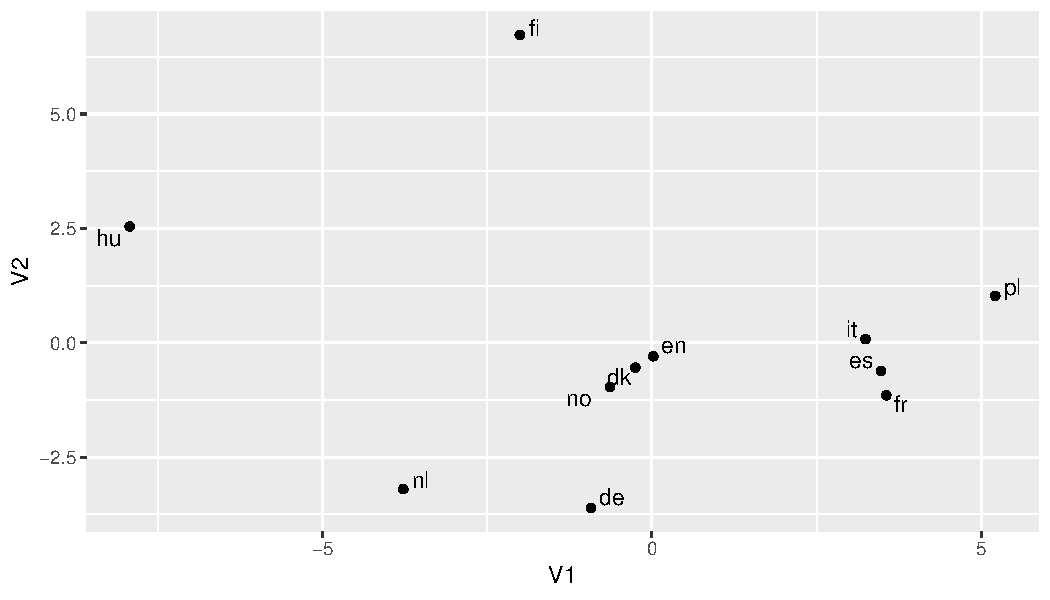
\includegraphics[width=\maxwidth]{figure/padova-1} 

\end{knitrout}
  
  
  
\end{frame}

\begin{frame}[fragile]{Comments}
  
  \begin{itemize}
  \item Tight clusters: Italian-Spanish-French, English-Danish-Norwegian.
  \item Dutch and German close to English group.
  \item Polish close to French group.
  \item Hungarian, Finnish distant from everything else and each other!
  \item Similar conclusions as from the cluster analysis.
  \end{itemize}
  
\end{frame}

\begin{frame}[fragile]{Shepard diagram}
  
  \begin{itemize}
  \item Stress for languages data was 5.3\%, very low.
  \item How do observed dissimilarities and map distances correspond?
  \item For low stress, expect larger dissimilarity to go with larger
    map distance, almost all the time.
  \item Not necessarily a linear trend since non-metric MDS works with
    \emph{order} of values.
  \item Actual dissimilarity on $x$-axis; map distances on $y$-axis.
  \end{itemize}
  
\end{frame}

\begin{frame}[fragile]{Shepard diagram for languages}
  
\begin{knitrout}
\definecolor{shadecolor}{rgb}{0.969, 0.969, 0.969}\color{fgcolor}\begin{kframe}
\begin{alltt}
\hlstd{lang.sh}\hlkwb{=}\hlkwd{Shepard}\hlstd{(d,number.nm}\hlopt{$}\hlstd{points)}
\hlkwd{ggplot}\hlstd{(}\hlkwd{as.data.frame}\hlstd{(lang.sh),}\hlkwd{aes}\hlstd{(}\hlkwc{x}\hlstd{=x,}\hlkwc{y}\hlstd{=y))}\hlopt{+}\hlkwd{geom_point}\hlstd{()}
\end{alltt}
\end{kframe}
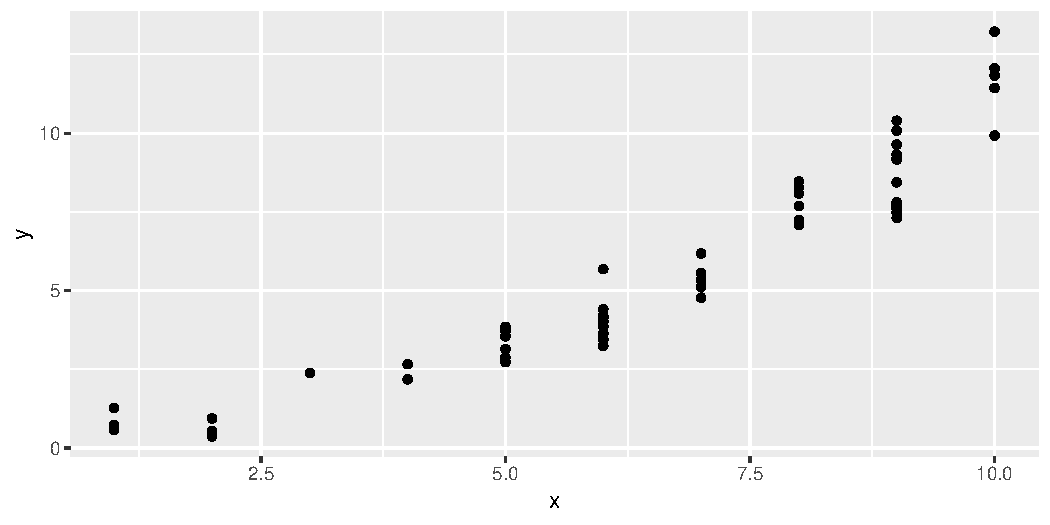
\includegraphics[width=\maxwidth]{figure/parma-1} 

\end{knitrout}
When actual dissimilarity $x$ between two languages higher, mapped
distance $y$ from MDS usually higher too. (MDS working well.)
  
\end{frame}

\begin{frame}[fragile]{Residuals}

  \begin{itemize}
  \item Actual distances in \texttt{d}. Make distance matrix of all
    the pairs of languages from their locations on map, then subtract
    from actual distances:
  {\small
\begin{knitrout}
\definecolor{shadecolor}{rgb}{0.969, 0.969, 0.969}\color{fgcolor}\begin{kframe}
\begin{alltt}
\hlstd{fitdist}\hlkwb{=}\hlkwd{dist}\hlstd{(number.nm}\hlopt{$}\hlstd{points)}
\hlkwd{round}\hlstd{(d}\hlopt{-}\hlstd{fitdist,}\hlnum{1}\hlstd{)}
\end{alltt}
\begin{verbatim}
##      en   no   dk   nl   de   fr   es   it   pl   hu
## no  1.1                                             
## dk  1.6  0.4                                        
## nl  2.2  1.2  1.6                                   
## de  2.6  1.3  1.9  2.1                              
## fr  2.4  1.8  2.1  1.4  1.9                         
## es  2.5  1.9  1.3  1.3  1.7  1.5                    
## it  2.8  2.0  1.5  1.3  1.4 -0.3  0.3               
## pl  1.6  0.8  0.3  0.1  0.3  2.3  0.6  1.8          
## hu  0.6 -0.1 -0.3  0.9 -0.3 -2.1 -1.8 -1.4 -3.2     
## fi  1.7  1.2  1.5 -1.1 -1.4 -0.6 -0.2 -0.5 -0.2  0.8
\end{verbatim}
\end{kframe}
\end{knitrout}
%$
}

\item English: many large positive residuals (farther from many
  languages than predicted).
\item Polish-Hungarian: large \emph{negative} residual.
    
  \end{itemize}
  
\end{frame}

\begin{frame}[fragile]{Cube, revisited}
  
\begin{knitrout}
\definecolor{shadecolor}{rgb}{0.969, 0.969, 0.969}\color{fgcolor}\begin{kframe}
\begin{alltt}
\hlstd{cube}\hlkwb{=}\hlkwd{read.table}\hlstd{(}\hlstr{"cube.txt"}\hlstd{,}\hlkwc{header}\hlstd{=T)}
\hlstd{cube.d}\hlkwb{=}\hlkwd{as.dist}\hlstd{(cube)}
\hlstd{cube.2}\hlkwb{=}\hlkwd{isoMDS}\hlstd{(cube.d,}\hlkwc{trace}\hlstd{=F) ; cube.2}\hlopt{$}\hlstd{stress}
\end{alltt}
\begin{verbatim}
## [1] 17.97392
\end{verbatim}
\begin{alltt}
\hlstd{cube.3}\hlkwb{=}\hlkwd{isoMDS}\hlstd{(cube.d,}\hlkwc{k}\hlstd{=}\hlnum{3}\hlstd{,}\hlkwc{trace}\hlstd{=F) ; cube.3}\hlopt{$}\hlstd{stress}
\end{alltt}
\begin{verbatim}
## [1] 0.007819523
\end{verbatim}
\end{kframe}
\end{knitrout}

\begin{itemize}
\item Stress is 18\% for 2 dimensions, basically 0\% for 3.
\item Three
  dimensions correct, two dimensions bad.
\item Shepard diagrams for these:
  
\begin{knitrout}\footnotesize
\definecolor{shadecolor}{rgb}{0.969, 0.969, 0.969}\color{fgcolor}\begin{kframe}
\begin{alltt}
\hlstd{cube2.sh}\hlkwb{=}\hlkwd{Shepard}\hlstd{(cube.d,cube.2}\hlopt{$}\hlstd{points)}
\hlstd{g2}\hlkwb{=}\hlkwd{ggplot}\hlstd{(}\hlkwd{as.data.frame}\hlstd{(cube2.sh),}\hlkwd{aes}\hlstd{(}\hlkwc{x}\hlstd{=x,}\hlkwc{y}\hlstd{=y))}\hlopt{+}\hlkwd{geom_point}\hlstd{()}
\hlstd{cube3.sh}\hlkwb{=}\hlkwd{Shepard}\hlstd{(cube.d,cube.3}\hlopt{$}\hlstd{points)}
\hlstd{g3}\hlkwb{=}\hlkwd{ggplot}\hlstd{(}\hlkwd{as.data.frame}\hlstd{(cube3.sh),}\hlkwd{aes}\hlstd{(}\hlkwc{x}\hlstd{=x,}\hlkwc{y}\hlstd{=y))}\hlopt{+}\hlkwd{geom_point}\hlstd{()}
\end{alltt}
\end{kframe}
\end{knitrout}
\end{itemize}
  
\end{frame}

\begin{frame}[fragile]{Shepard diagram for 2-dimensional cube}

\begin{knitrout}
\definecolor{shadecolor}{rgb}{0.969, 0.969, 0.969}\color{fgcolor}\begin{kframe}
\begin{alltt}
\hlstd{g2}
\end{alltt}
\end{kframe}
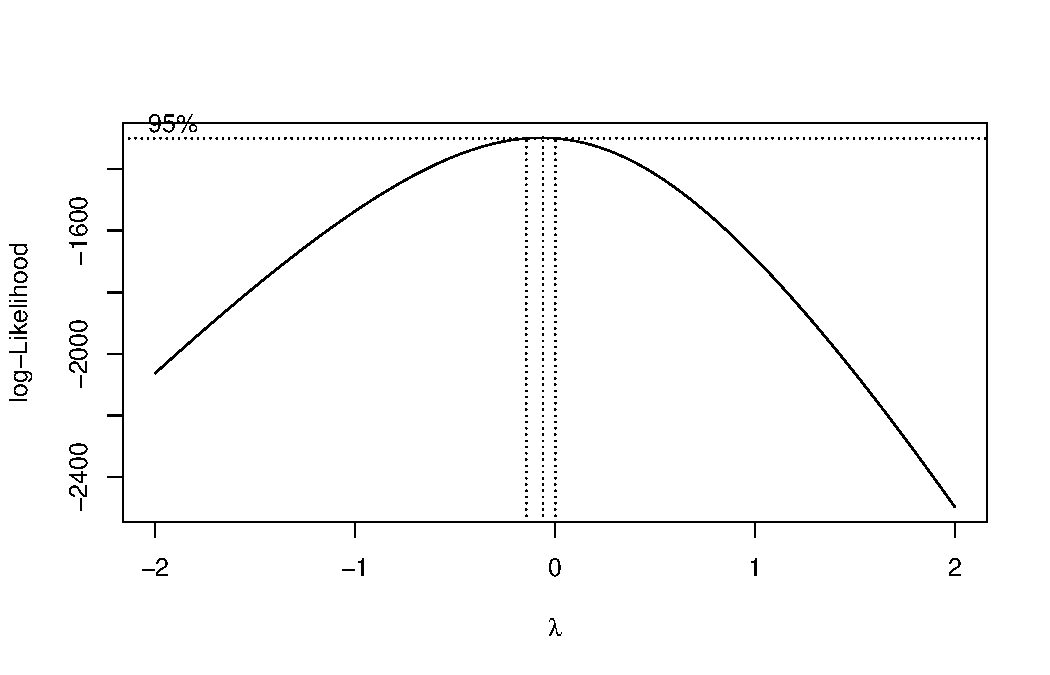
\includegraphics[width=\maxwidth]{figure/unnamed-chunk-38-1} 

\end{knitrout}

Poor correspondence (not much trend).
\end{frame}

\begin{frame}[fragile]{Shepard diagram for 3-dimensional cube}
  
\begin{knitrout}
\definecolor{shadecolor}{rgb}{0.969, 0.969, 0.969}\color{fgcolor}\begin{kframe}
\begin{alltt}
\hlstd{g3}
\end{alltt}
\end{kframe}
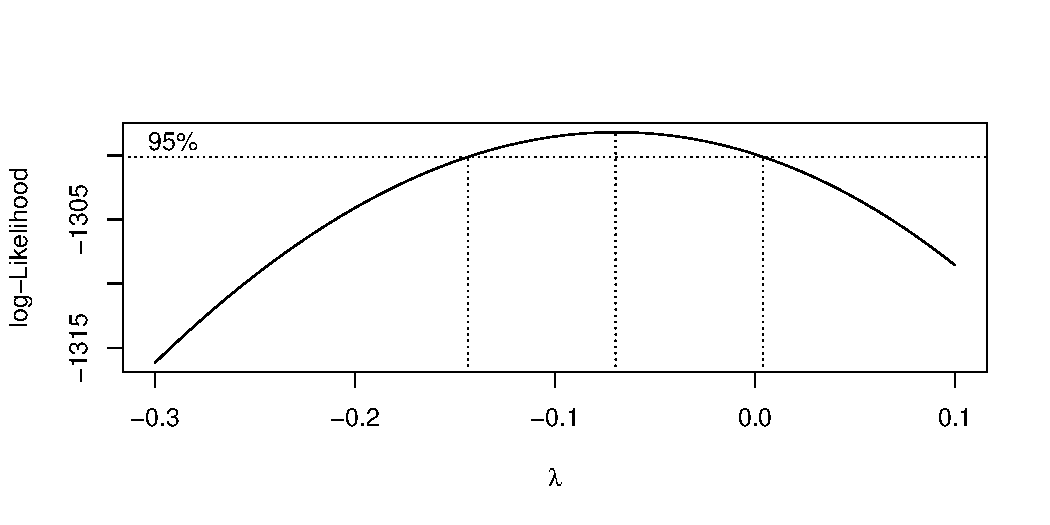
\includegraphics[width=\maxwidth]{figure/unnamed-chunk-39-1} 

\end{knitrout}
  
Almost perfect: all actual $x=1$ go with smallest mapped distances; almost
all $x=1.7$ go with  largest.
\end{frame}

\begin{frame}[fragile]{Guidelines for stress values, in \%}

Smaller is better:


\begin{tabular}{lp{3in}}
  Stress value & Interpretation \\
  \hline
  Less than 5 & Excellent: no prospect of misinterpretation (rarely achieved)\\
  5--10 & Good: most distances reproduced well, small prospect of false inferences\\
10--20 & Fair: usable, but some distances misleading.\\
More than 20 & Poor: may be dangerous to interpret\\
\hline
\end{tabular}

\begin{itemize}
\item Languages: stress in ``good'' range.
\item Cube: 
  \begin{itemize}
  \item   2 dimensions ``fair'', almost ``poor'';
  \item 3 dimensions, ``excellent''.
  \end{itemize}
\end{itemize}
  
\end{frame}

